\documentclass{llncs}
\usepackage{makeidx}
\usepackage[spanish]{babel}
\usepackage[utf8]{inputenc}
\usepackage{amsmath}
\usepackage{url}
\usepackage{fancyvrb}
\usepackage{babelbib}
\usepackage{graphicx}

\graphicspath{ {img/} }

\urldef{\mails}\path|{fbarrios,fjlopez}@fi.uba.ar| 

\newtheorem{definicion}{Definición} 

\begin{document}

\frontmatter
\pagestyle{headings}

\title{Variantes de TextRank para la Generación de Resúmenes Automáticos}
\titlerunning{Variantes de TextRank} 

\author{Luis Argerich \and Federico Barrios \and Federico López}
\institute{Facultad de Ingeniería, Universidad de Buenos Aires,\\
Av. Paseo Colón 850, Ciudad Autónoma de Buenos Aires, Argentina\\
\mails\\
\url{http://ingenieria.uba.ar/}}

\maketitle

\begin{abstract}
Lorem ipsum dolor sit amet, consectetur adipiscing elit. Nullam nec dictum 
nibh, vel lacinia lectus. Morbi non mi mattis, accumsan arcu id, venenatis 
eros. Nunc est ex, efficitur hendrerit posuere eget, dapibus at orci. 
Cras feugiat erat ut volutpat blandit. Aliquam erat volutpat. Mauris 
auctor congue libero et aliquet. Etiam justo mi, tempor sit amet feugiat 
ut, tincidunt id augue. Pellentesque quis nibh vel turpis mattis dignissim. 
Duis elementum sem quam, eget dignissim nibh suscipit a. Fusce quis magna 
eu neque efficitur ornare nec sed turpis. Aenean mollis ipsum tristique vestibulum tempus. 
Sed in ornare ipsum. Vivamus purus mi, sollicitudin.
\keywords{variantes, TextRank, generación, resúmenes, automáticos}

\end{abstract}

\section{Introducción}
Foo bar baz

\section{Trabajo previo}
Se ha visto un gran avance en el campo de la generación automática de resúmenes desde finales de 1960 hasta la actualidad \cite{miranda}. Los métodos tradicionales tienen en cuenta la frecuencia de palabras o frases introductorias para identificar las oraciones más sobresalientes del texto. Asimismo, se han desarrollado modelos estadísticos basados en corpus de entrenamiento para combinar diferentes heurísticas: palabras clave, posición y longitud de las oraciones, frecuencia de palabras y contenido de los títulos \cite{hovy}. Otros enfoques se basan en la representación del texto en forma de grafo: las oraciones importantes y los conceptos son las entidades altamente conectadas y, por esto, forman parte del resumen \cite{barzilay}. De igual modo, se ha propuesto analizar la estructura discursiva y extraer las relaciones retóricas entre las diferentes unidades textuales, y así separar las principales de las secundarias para descubrir aquéllas que juegan un papel preponderante \cite{marcu}.

En la línea de representación del texto como un grafo conectado se usan técnicas de Recuperación de Información para identificar oraciones similares y determinar las más importantes, que formarán al resumen final \cite{salton}. El enfoque propuesto, tanto por Mihalcea y Tarau como por Erkan y Radev \cite{erkan}, consiste en utilizar el prestigio de las unidades léxicas (oraciones o palabras) dentro del grafo. Dicha técnica es la que adopta el algoritmo de TextRank.


\section{TextRank}

\subsection{Descripción}
TextRank es un algoritmo no supervisado basado en grafos para realizar resúmenes automáticos extractivos u obtener palabras claves de un texto. Fue presentado en 2004 por Rada Mihalcea y Paul Tarau en la publicación “TextRank: Bringing Order into Texts” \cite{mihalcea-tarau}.

El algoritmo aplica una variación de PageRank \cite{pageetal98} sobre un grafo especialmente diseñado para la tarea. De esta manera permite explotar la estructura del texto, identificando los conceptos principales, sin necesidad de datos previos de entrenamiento. Debido a que se basa en PageRank, se sirve de la noción del “prestigio” o “recomendación” entre los elementos del grafo, lo que lo hace aplicable a cualquier texto incluso sin importar el idioma.

El algoritmo modela el texto en base a un grafo, y luego busca crear relaciones significativas (aristas) entre las entidades léxicas (vértices). Dependiendo de la aplicación que se desee dar al algoritmo, las entidades pueden ser palabras, frases, oraciones, párrafos, entre otros. De manera similar, también debe definirse el tipo de relación que se usa para unir los vértices: semántica, contextual, de superposición, y demás.

Los pasos principales que se llevan a cabo son los siguientes:

\begin{enumerate}
\item Identificar las unidades del texto (palabras u oraciones) y agregarlas al grafo como vértices.
\item Identificar relaciones que conectan a estas unidades, y agregarlas al grafo como aristas entre los vértices. Las aristas pueden ser dirigidas o no, y ponderadas o no.
\item Aplicar PageRank para asignarle un puntaje a cada vértice.
\item Ordenar los vértices de acuerdo al puntaje y utilizarlo para armar el resumen de acuerdo a algún criterio.
\end{enumerate}

\subsection{Generación de resúmenes automáticos}
El problema de la extracción de oraciones apunta a identificar las secuencias más representativas del texto. Para este caso, las unidades tomadas para aplicar el algoritmo serán oraciones completas \cite{introductionir}.

Inicialmente, se construye un grafo en base al texto. Cada oración se considera como un vértice, y para asignarles peso a las aristas se debe definir una función de similitud entre dos oraciones dadas. Esta función será la que dicte cuánto una oración “recomienda” a otra, dependiendo de la similitud entre sus contenidos por abordar los mismos conceptos.
    
La función utilizada se define formalmente de la siguiente manera:


\begin{definicion}
Sean $S_i$, $S_j$ dos oraciones representadas por un conjunto de $n$ palabras que en 
$S_i$ aparecen como $S_i = w_{1}^{i}, w_{2}^{i},..., w_{n}^{i}$. La función de similitud para $S_i$, $S_j$ se define como:


\begin{equation}
Similitud(S_{i},S_{j}) = \frac{ | \{   w_{k} | w_{k} \in S_{i} \& w_{k} \in S_{j}   \}  | }    
                              {  log(|S_{i}|) + log(|S_{j}|)  }
\end{equation}


\end{definicion}
    
El resultado de este proceso es el texto representado como un grafo ponderado y altamente conexo. En base a esto se aplica PageRank para priorizar los vértices más relevantes.

Luego de aplicar el algoritmo de priorización se seleccionan las oraciones con mayor puntaje para incluirlas en el resumen. Estas, finalmente, se presentan de acuerdo al orden de aparición en el texto original.


\section{Experimentos}

\subsection{Evaluación}
Se decidió usar la base de datos de la tarea de generación de resúmenes automáticos de la conferencia DUC (Document Understanding Conference) del año 2002, al igual que en la publicación original. El corpus cuenta de 567 documentos que fueron resumidos a cerca del 20\%.

Para llevar a cabo la evaluación se usó la versión 1.5.5 del paquete de métricas ROUGE \cite{Lin2004a}. Se utilizó la configuración usada en DUC, calculando sólo las mediciones ROUGE-1, ROUGE-2 y ROUGE-SU4 en un intervalo de confianza del 95\% y aplicando un método de \textit{stemming}. Se obtuvo un único puntaje promediando los tres valores.

Para verificar el funcionamiento de todo el conjunto se implementó el método de referencia (\textit{baseline}) usado en la publicación, que construye el resumen extrayendo las primeras oraciones de cada artículo. Se comprobó que los resultados fueron similares: la versión original de TextRank mejora al \textit{baseline} por cerca de un 2,3\%.

\subsection{Propuestas}

\subsubsection{Subcadena común}
Dadas dos frases, el problema de la subcadena común más larga consiste en identificar la secuencia de caracteres de mayor extensión presente en ambas. Por ejemplo, entre “la cocina verde” y “una cocina vale más si es verde”, la secuencia más larga es “a cocina v”.

La propuesta consiste en modificar la función de distancia de la implementación original y reemplazarla por el largo de la subcadena común más larga. En el ejemplo anterior, la similitud sería de 10, dado que es el largo de la secuencia “a cocina v”.

Cabe destacar el parecido de esta métrica con los métodos de evaluación ROUGE.


\subsubsection{Similitud coseno}
La similitud coseno es una medida de la similitud existente entre dos vectores en un espacio que posee un producto interior con el que se evalúa el valor del coseno del ángulo comprendido entre ellos. Para poder hacer uso de esta “distancia” se utiliza el modelo del espacio vectorial, y así modelar a los documentos como vectores.

Este modelo algebraico es utilizado para representar documentos en lenguaje natural de una manera formal mediante el uso de vectores en un espacio lineal multidimensional. La teórica básica es que el parecido de un documento frente a otro puede calcularse usando la similitud coseno. Así un valor de coseno de cero significa que los documentos son ortogonales el uno al otro, y eso significa que no hay similitud.

La propuesta se basa en aplicar este modelo para tratar a cada oración del texto como un vector n-dimensional (con n la cantidad de palabras distintas presentes en el documento), y luego compararlas utilizando la similitud coseno. Las entradas de cada vector estarán compuestas por el resultado de aplicar la función “frecuencia de término -- frecuencia inversa de documento” (TF--IDF de sus siglas en inglés) a cada palabra de la oración representada.

Tomando como ejemplo el documento “Esta bien. Todo bien.”, las oraciones quedarían modeladas como vectores de la siguiente forma:

\begin{Verbatim}[xleftmargin=3em]
v1=[ TFIDF("Esta") , TFIDF("bien") ,       0       ]
v2=[       0       , TFIDF("bien") , TFIDF("Todo") ]
\end{Verbatim}

Dado que la imagen de la función TFIDF está contenida en el intervalo [0,1], todos los vectores quedan conformados por entradas no negativas, haciendo que ninguna similitud sea menor a cero. 


\subsubsection{BM25}
Okapi BM25 es una función de ranking utilizada para la asignación de relevancia a los documentos en un buscador. 
Está basada en los modelos probabilísticos de Recuperación de información, y actualmente 
representa el estado del arte en algoritmos de recuperación de documentos 
basados en frecuencia de término -- frecuencia inversa de documento.

\begin{definicion}
Dadas dos oraciones R, S, BM25 se define como:

\begin{equation}
BM25(R,S) = \sum_{i=1}^{n} IDF(s_i) \cdot \frac{f(s_i, R) \cdot (k_1 + 1)}{f(s_i, R) + k_1 \cdot (1 - b + b \cdot \frac{|R|}{avgDL})}
\end{equation}

donde $k$ y $b$ son parámetros que valen $k = 1,2$ y $b = 0,75$, y $avgDL$ es el largo promedio de las oraciones en el texto.
\end{definicion}

Esta función contempla la frecuencia inversa del documento de manera tal que si una palabra aparece en más de la mitad de los textos, el valor para ese término se vuelve negativo. Dado que este comportamiento no es deseable para esta aplicación, se utiliza la siguiente fórmula:
                
\begin{equation}
 IDF(q_i) =
  \begin{cases}
       log(N - n(q_i) + 0.5) - log(n(q_i) + 0.5)    & \text{si }  n(q_i) > N/2\\
       \varepsilon \cdot avgIDF                     & \text{si }  n(q_i) \leq N/2\\
  \end{cases}
\end{equation}                
                
donde $\varepsilon$ ronda entre 0,5 y 0,30 y $avgIDF$ es el idf promedio para todos los términos.
También se ensayaron alternativas como igualar a cero el resultado en caso de ser negativo, o reemplazar la función inversa por una similar, cuyo resultado es no negativo, o estrictamente positivo. 

Existe una variante a BM25 llamada BM25+. Esta repara deficiencias relacionadas a la frecuencia de término y a la penalización a documentos largos frente a documentos cortos irrelevantes.

La propuesta consistió en aplicar BM25 y BM25+ entre las oraciones de un texto, a fin de ordenarlas de acuerdo a su relevancia.


\subsection{Resultados}
Los mejores resultados se obtuvieron usando BM25 y BM25+. El incremento más alto se logró al reemplazar los valores negativos por la constante $\varepsilon$ = 0.25, dando una mejora total de 2,92\% para BM25 y 2,60\% para BM25+. Inicialmente se obtuvieron valores cercanos al 1,30\%, pero dado que esta función contempla el uso de \textit{stopwords} se procedió a eliminar la etapa de filtrado del preprocesamiento del texto, alcanzado así resultados sobresalientes. En el Cuadro 1 se detallan las alternativas ensayadas.

\begin{table}
\caption{Resultados de las distintas propuestas}
\begin{center}
\begin{tabular}{l*{5}{c}r}
\hline
\rule{0pt}{12pt}
Método & ROUGE-1 & ROUGE-2 & ROUGE-SU4 & Mejora \\[2pt]
\hline\rule{0pt}{12pt}\mbox{}\par\nobreak
BM25 (Neg a epsilon) & 0.4042 & 0.1831 & 0.2018 & 2,92\% \\
BM25+ (Neg a epsilon) & 0.404 & 0.1818 & 0.2008 & 2,60\% \\
Cosine TF-IDF & 0.4108 & 0.177 & 0.1984 & 2,54\% \\
BM25+ (IDF = log(N/NI)) & 0.4022 & 0.1805 & 0.1997 & 2,05\% \\ 
BM25 (IDF = log(N/NI)) & 0.4012 & 0.1808 & 0.1998 & 1,97\% \\ 
Longest Common Substring & 0.402 & 0.1783 & 0.1971 & 1,40\% \\
BM25+ (Neg a cero) & 0.3992 & 0.1803 & 0.1976 & 1,36\% \\ 
BM25 (Neg a cero) & 0.3991 & 0.1778 & 0.1966 & 0,89\% \\
\textbf{TextRank} & \textbf{0.3983} & \textbf{0.1762} & \textbf{0.1948} & \textbf{-}\\
BM25 & 0.3916 & 0.1725 & 0.1906 & -1,57\% \\
BM25+ & 0.3903 & 0.1711 & 0.1894 & -2,07\% \\
DUC Baseline & 0.39 & 0.1689 & 0.186 & -2,84\% \\ [2pt]
\hline
\end{tabular}
\end{center}
\end{table}

Los tiempos de ejecución también se superaron. Se pudo procesar los 567 documentos de la base de datos de DUC2002 utilizando 84\% del tiempo requerido por la versión original.

El resultado de la métrica de similitud coseno también fue satisfactoria, presentando una mejora de 2,54\% por sobre el método original. A su vez, los métodos de secuencias de máxima longitud también mostraron una mejora considerable: cerca del 1,40\% por sobre TextRank. En la Figura 1 se comparan los distintas técnicas.

\begin{figure}[h!]
    \centering
    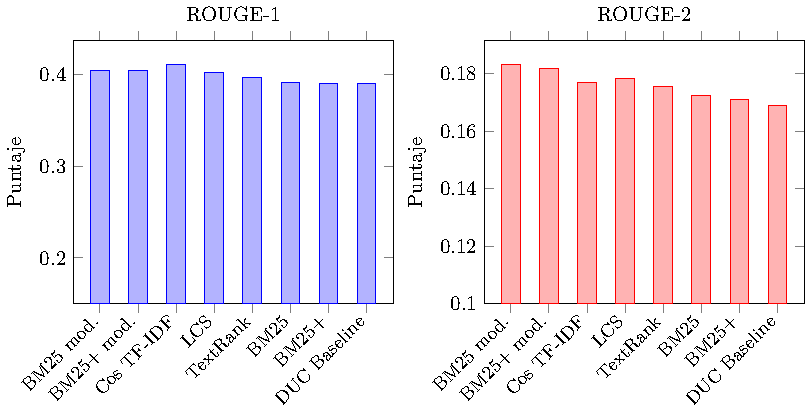
\includegraphics[width=1\textwidth]{rouge-scores.pdf}
    \caption{Comparación de métricas.}
\end{figure}

\section{Conclusiones}
En este trabajo se analizaron variantes al algoritmo de TextRank. A partir del mismo se propusieron e implementaron optimizaciones cuyos resultados fueron significativos: se obtuvo una mejoría del 2,92\% por sobre el método original. Este número es notable si se tiene en cuenta que TextRank por sí solo performa 2,84\% por sobre el estándar de comparación.

Las evaluaciones fueron hechas con las mismas técnicas y conjuntos de datos utilizados en competencias internacionales, validando así las mediciones.

Queda para próximos trabajos explorar alternativas para la extracción de palabras claves, y el ensayo de distintos métodos algebraicos, haciendo uso del modelo del espacio vectorial.


\bibliography{report}{}
\bibliographystyle{babunsrt}


\end{document}
